\documentclass[12pt]{article}
\usepackage[margin=3cm]{geometry}
\usepackage{graphicx}
\usepackage{float}
\usepackage{url}
\usepackage{listings}
\usepackage{color}

\definecolor{mygreen}{rgb}{0,0.6,0}
\definecolor{mygray}{rgb}{0.5,0.5,0.5}
\definecolor{mymauve}{rgb}{0.58,0,0.82}
\lstset{ %
	xleftmargin=2em,
	backgroundcolor=\color{white},   % choose the background color; you must add \usepackage{color} or \usepackage{xcolor}
	basicstyle=\small,%\footnotesize,        % the size of the fonts that are used for the code
	breakatwhitespace=false,         % sets if automatic breaks should only happen at whitespace
	breaklines=true,                 % sets automatic line breaking
	captionpos=b,                    % sets the caption-position to bottom
	commentstyle=\color{mygreen},    % comment style
	deletekeywords={...},            % if you want to delete keywords from the given language
	escapeinside={\%*}{*)},          % if you want to add LaTeX within your code
	extendedchars=true,              % lets you use non-ASCII characters; for 8-bits encodings only, does not work with UTF-8
	%	frame=single,                    % adds a frame around the code
	keepspaces=true,                 % keeps spaces in text, useful for keeping indentation of code (possibly needs columns=flexible)
	keywordstyle=\color{blue},       % keyword style
	language=verilog, % the language of the code
	morekeywords={*,...},            % if you want to add more keywords to the set
	numbers=left,                    % where to put the line-numbers; possible values are (none, left, right)
	numbersep=5pt,                   % how far the line-numbers are from the code
	numberstyle=\small\color{mygray}, % the style that is used for the line-numbers
	rulecolor=\color{black},         % if not set, the frame-color may be changed on line-breaks within not-black text (e.g. comments (green here))
	showspaces=false,                % show spaces everywhere adding particular underscores; it overrides 'showstringspaces'
	showstringspaces=false,          % underline spaces within strings only
	showtabs=false,                  % show tabs within strings adding particular underscores
	stepnumber=1,                    % step between two line-numbers. If it's 1, each line will be numbered
	stringstyle=\color{mymauve},     % string literal style
	tabsize=2                  % sets default tabsize to 2 spac                  % show the filename of files included with \lstinputlisting; also try caption instead of title
}

\begin{document}

\begin{titlepage}
	\begin{center}
		
		
		% Upper part of the page. The '~' is needed because \\
		% only works if a paragraph has started.
		\vfill
		
		\textsc{\LARGE Case Study for 32-Bit Pipelined CPU\\[0.2cm] Design with New ALU Architecture}\\[1.5cm]
		
		\Large Adam Sumner\\[0.5cm]
		
		\Large Illinois Institute of Technology\\[0.5cm]
		
		\Large ECE 429-01\\[0.5cm]
		
		\Large December 4\textsuperscript{th}, 2015	
		
		\noindent
		\vfill
		%\large \textbf{Lab Date:} November 9\textsuperscript{th}, 2015\hfill
		%\large \textbf{Due Date:} November 18\textsuperscript{th}, 2015
		% Bottom of the page
	
		
	\end{center}
\end{titlepage}
\tableofcontents
\newpage
\section{Introduction}
The objective of this project is to understand how a 32-bit pipelined Central Processing Unit (CPU) functions and how it is both physically and logically constructed. As the name suggests, the length of a word is 32 bits wide. Furthermore, due to the wonderful invention of pipelining, multiple instructions can be executed simultaneously. A CPU's normal processes (excluding interrupts) are synchronized, therefore the CPU will be in sync using an external clock signal. The instruction signals for addressing the memory file, Arithmetic Logic Unit (ALU) operands, and the ALU operation are also external. 

\subsection{Circuit Description}
The complete overview of the primary building blocks and signals of the CPU are shown in Figure \ref{fig:overview}. The two main components are the memory file and the ALU. The external clock signal synchronizes the capture and release of data within the 32 x 32 memory file block. Because of pipelining, each instruction executed can be performed in 2 clock cycles. The first cycle involves the two decoders translating the external address selection signals used for specifying the contents of the memory file that should be read. In addition to this, the multiplexer blocks are used to select the operands for the ALU. In the second clock cycle, the ALU performs the specified operation. The output of the ALU can then be read from outside the CPU through a tri-state buffer, and they can also be written back into the memory file in the word specified by Address B.
\begin{figure}[H]
\centering
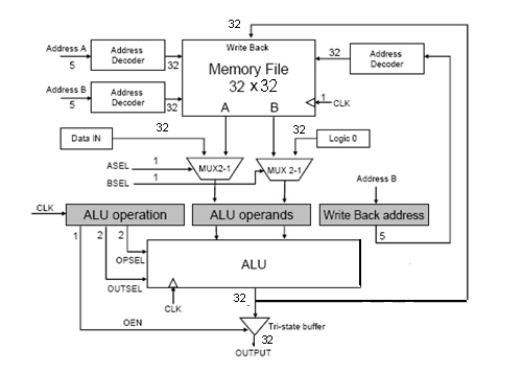
\includegraphics[width=0.7\linewidth]{overview}
\caption{Circuit Overview}
\label{fig:overview}
\end{figure}

\subsection{Memory File}
The memory file stores 32 32-bit words. There are two read ports and one write port. The words that are read in each clock cycle are specified in Address A and Address B from Figure \ref{fig:overview}. The primary storage element used in this design is a D-register. The output of each register is connected to the two output read ports through tri-state buffers. The buffers are enabled through the decoded address A and address B. The value of address B specifies the word address in the memory file where the results of the ALU will be stored after the computation is complete in the second clock cycle.

\begin{figure}[H]
	\centering
	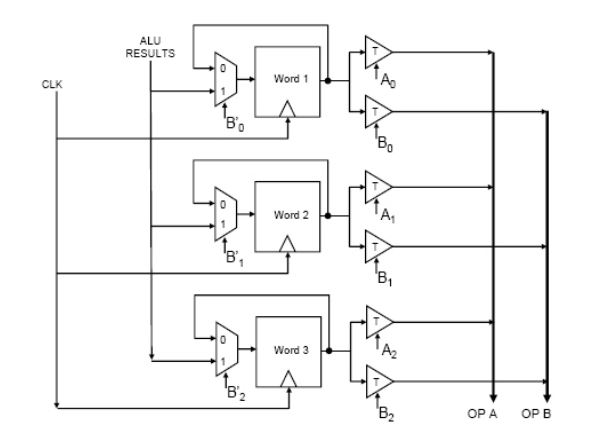
\includegraphics[width=0.7\linewidth]{memory-file}
	\caption{Memory File}
	\label{fig:memory-file}
\end{figure}
\subsection{ALU}
The ALU of the circuit has two operands A and B, and it implements the following functions:
\begin{itemize}
	\item A * B : multiplication
	\item A + B : addition
	\item A - B : subtraction
	\item B - A : subtraction
	\item A or B : logic OR function
	\item A and B : logic AND function
	\item A xor B: exclusive XOR function
	\item A xnor B : logic XNOR function
\end{itemize}

The ALU has three primary operation blocks: the multiplier, the adder, and the logic function block. This is shown in figure \ref{fig:alu-overview}. The multiplier carries out the multiplication function. Because multiplication results in a 64-bit result, 2 clock cycles are used to store the result. This means that to execute the multiply instruction, 3 cycles instead of 2 are used in total.
\begin{figure}[H]
\centering
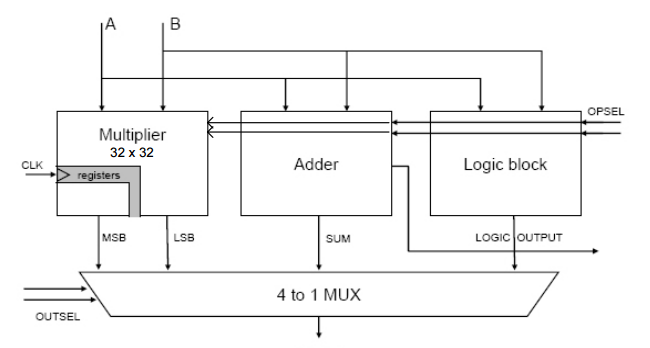
\includegraphics[width=0.7\linewidth]{alu-overview}
\caption{ALU Overview}
\label{fig:alu-overview}
\end{figure}
The adder circuit within the ALU is a 32-bit adder/subtractor circuit. It executes the addition and subtraction operations. The selection of the operation is done by the two externally defined operation select signals OPSEL. The same signals are used to specify the operation executed within the logic function of the ALU. The final output select signal OUTSEL specifies the result of the ALU for output using the 4-to-1 multiplexer.

\subsection{Synchronization}
Each instruction executed by the CPU is determined by the external control signals. An instruction word is shown in Figure \ref{fig:instruc}. Once the clock signals high, the instruction is applied to the signals that control the CPU operation. Since each instruction is executed in two steps, some control signals need to be stored at the internal registers of the CPU. In the first step of the instruction, the instruction specifies the contents of the memory file that will be read from the read ports A and B, and the operands of the ALU. In the second cycle, the control signals determine the operation to be executed internally in the ALU and the ALU output. The results of the ALU will be available if the OEN signal is set, and the result will also be written back into the memory file. This address is specified by address B. Data is written at the next positive edge of the clock. The period of the clock signal is determined by the longest data path delay in the circuit.
\begin{figure}[H]
\centering
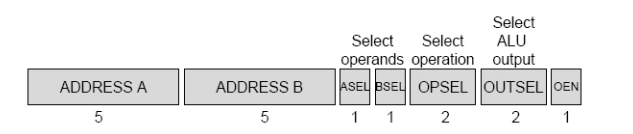
\includegraphics[width=0.7\linewidth]{instruc}
\caption{Instruction Word Contents}
\label{fig:instruc}
\end{figure}

\section{32-Bit CPU Design with Different Adders}

\subsection{Introduction}
The objective of this project is to carry out the logical and physical synthesis of a 32-bit cpu using 4 separate types of adder circuits. 
\subsection{Carry Ripple Adder}
An n-bit CRA is formed by concatenating n full adders in cascade with the carry output from one adder connected to the carry input of the next. This is shown in Figure \ref{fig:carry-ripple}.
\begin{figure}[H]
\centering
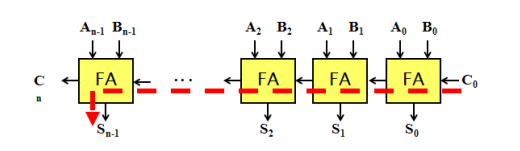
\includegraphics[width=0.7\linewidth]{carry-ripple}
\caption{Carry Ripple Adder}
\label{fig:carry-ripple}
\end{figure}

\subsubsection{RTL Simulation}
Figures \ref{fig:CRA-text} and \ref{fig:CRA-test} show the display and simvision results of the RTL simulation. The detailed results are included with this report under the CRA directory in the file \texttt{stim\_proj.out}.
\begin{figure}[H]
\centering
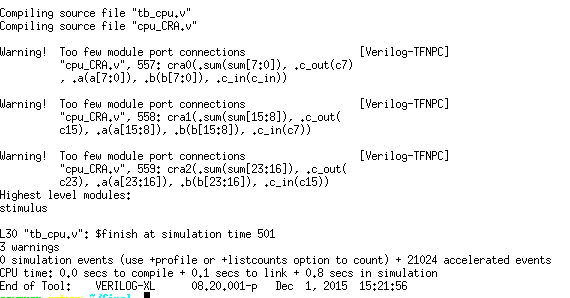
\includegraphics[width=.7\linewidth]{../CRA/CRA-text}
\caption{Display}
\label{fig:CRA-text}
\end{figure}
\begin{figure}[H]
\centering
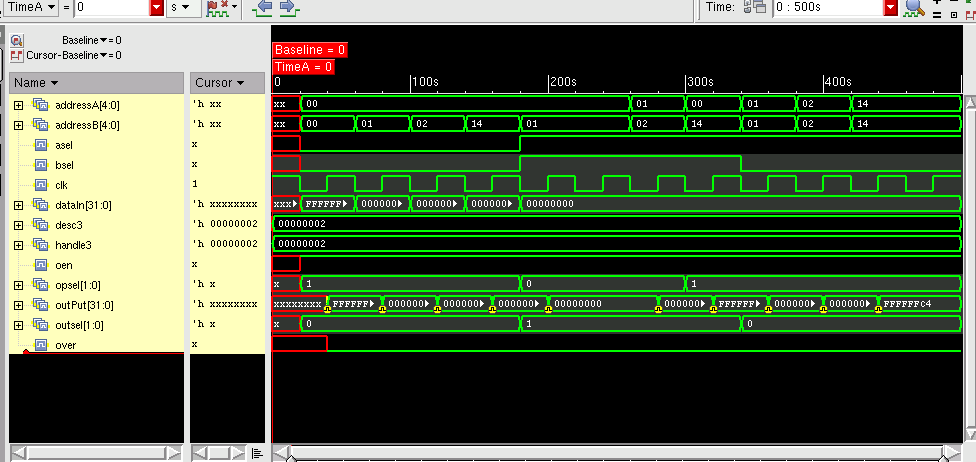
\includegraphics[width=\linewidth]{../CRA/CRA-test}
\caption{Simvision}
\label{fig:CRA-test}
\end{figure}

\subsubsection{Logic Synthesis and Post-Synthesis Simulation}
Figures \ref{fig:synth-text-CRA} and \ref{fig:synth-test-CRA} show the display and simvision results of the simulation. The results are included under the CRA directory under the files \texttt{timing.rep} and \texttt{cell.rep}. They show that this design uses 48610.093084nm of area and has a slack time of 26.14 meaning that the clock rate can be increased.
\begin{figure}[H]
\centering
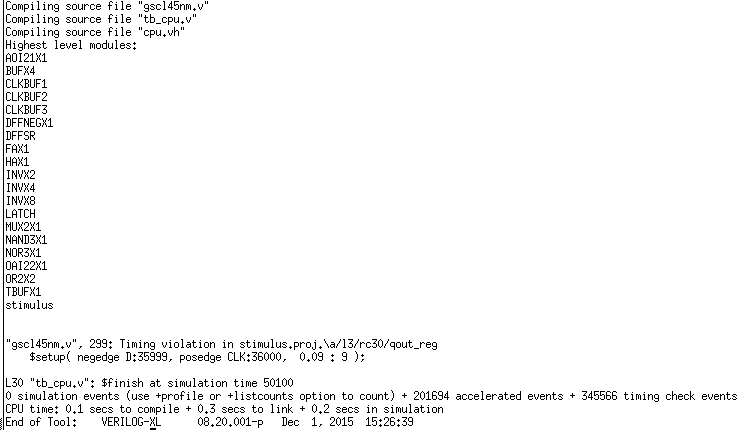
\includegraphics[width=.7\linewidth]{../CRA/synth-text}
\caption{Display}
\label{fig:synth-text-CRA}
\end{figure}
\begin{figure}[H]
\centering
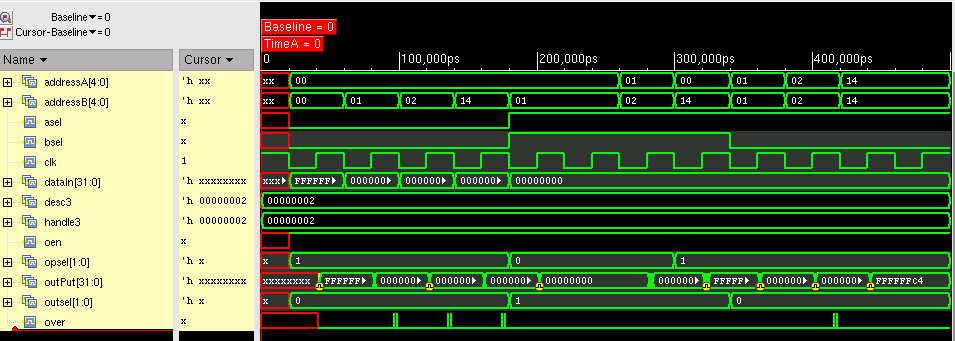
\includegraphics[width=\linewidth]{../CRA/synth-test}
\caption{Simvision}
\label{fig:synth-test-CRA}
\end{figure}

\subsubsection{Place \& Route and Post-P\&R Simulation}
Figures \ref{fig:encounter-text-CRA} and \ref{fig:encounter-test-CRA} show the display and simvision results. The file \texttt{timing.rep.5.final} is located under the CRA directory included with this report. It shows that the slack time is about 17.458 which is an improvement from the post-synthesis design, but the clock can still be increased. The max clock rate was found to be $\approx$ 62 MHz.
\begin{figure}[H]
\centering
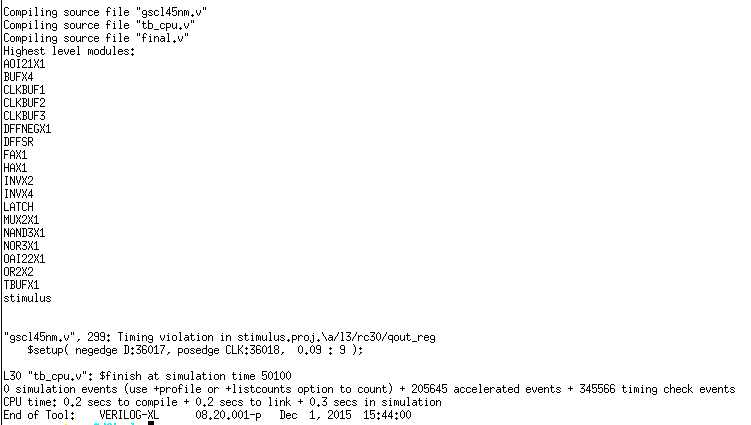
\includegraphics[width=.7\linewidth]{../CRA/encounter-text}
\caption{Display}
\label{fig:encounter-text-CRA}
\end{figure}
\begin{figure}[H]
\centering
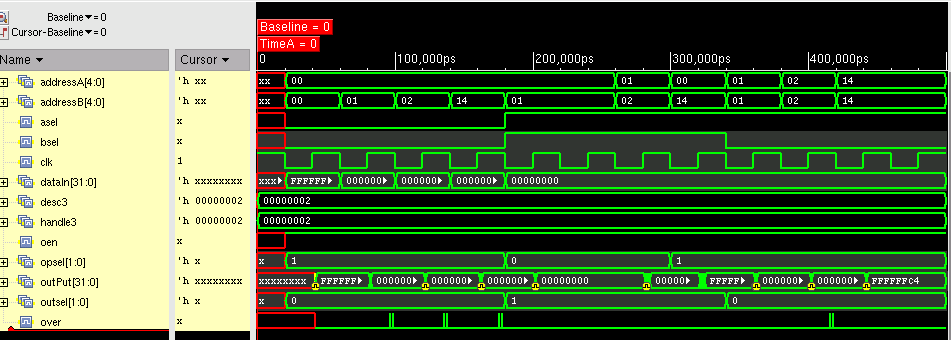
\includegraphics[width=1\linewidth]{../CRA/encounter-test}
\caption{Simvision}
\label{fig:encounter-test-CRA}
\end{figure}

\subsubsection{Test Bench}
Figures \ref{fig:test-text-CRA} and \ref{fig:test-test-CRA} show the display and simvision results. For a detailed analysis of the output please refer to the file \texttt{stim\_proj\_CRA.out} located under the CRA directory included with this report. Figures  \ref{fig:alu1-CRA} and \ref{fig:alu2-CRA} show a detailed view of the ALU results.

\begin{figure}[H]
\centering
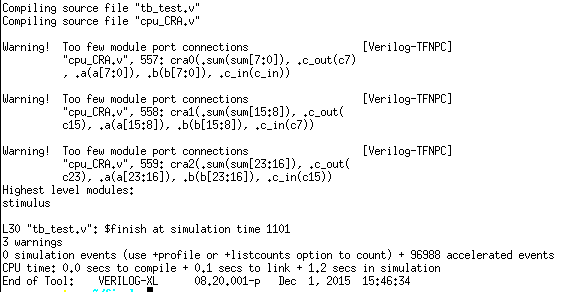
\includegraphics[width=.7\linewidth]{../CRA/test-text}
\caption{RTL Display}
\label{fig:test-text-CRA}
\end{figure}

\begin{figure}[H]
\centering
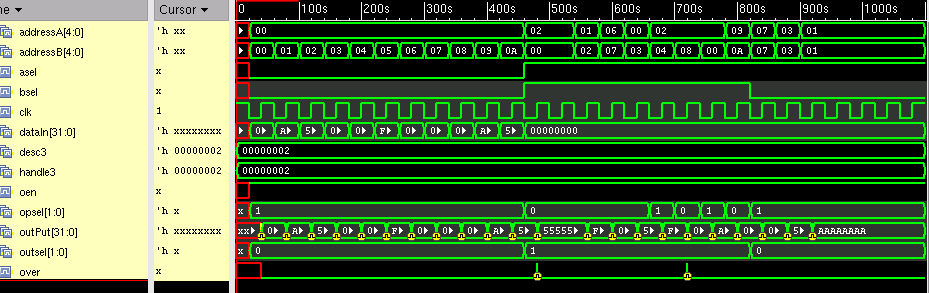
\includegraphics[width=1\linewidth]{../CRA/test-test}
\caption{RTL Simvision}
\label{fig:test-test-CRA}
\end{figure}


\begin{figure}[H]
\centering
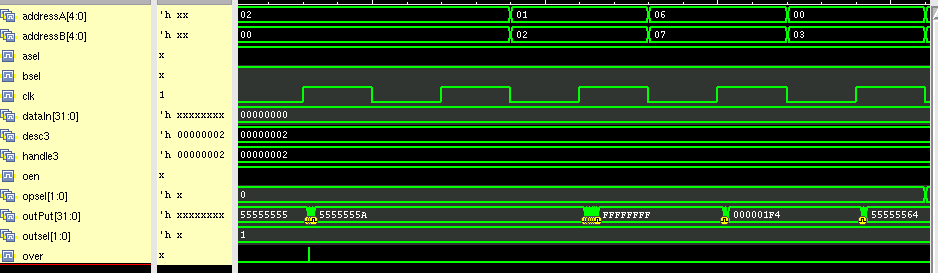
\includegraphics[width=\linewidth]{../CRA/alu1-test}
\caption{ALU Operations}
\label{fig:alu1-CRA}
\end{figure}

\begin{figure}[H]
\centering
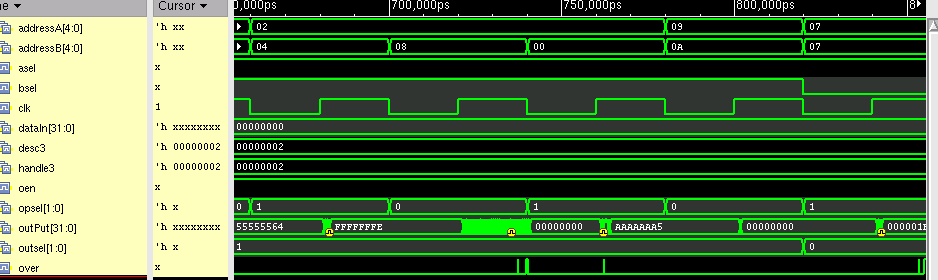
\includegraphics[width=1\linewidth]{../CRA/alu2-test}
\caption{ALU Operations}
\label{fig:alu2-CRA}
\end{figure}

\subsection{Carry Lookahead Adder}
Carry Lookahead circuits are special logic circuits that can dramatically reduce the time to perform addition at the price of more complex hardware. This is done by transforming the ripple carry design so that the carry logic over a fixed group of bits are reduced to two-level logic. This is shown in Figure \ref{fig:carry-lookahead}.
\begin{figure}[H]
\centering
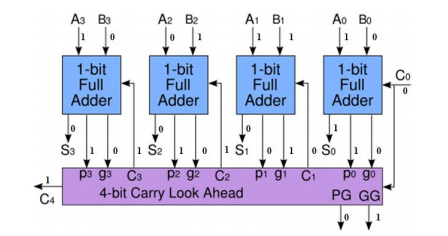
\includegraphics[width=0.7\linewidth]{carry-lookahead}
\caption{Carry Lookahead Adder}
\label{fig:carry-lookahead}
\end{figure}

\subsubsection{RTL Simulation}
Figures \ref{fig:CLA-text} and \ref{fig:CLA-test} show the display and simvision results of the RTL simulation. The detailed results are included with this report under the CRA directory in the file \texttt{stim\_proj.out}.

\begin{figure}[H]
\centering
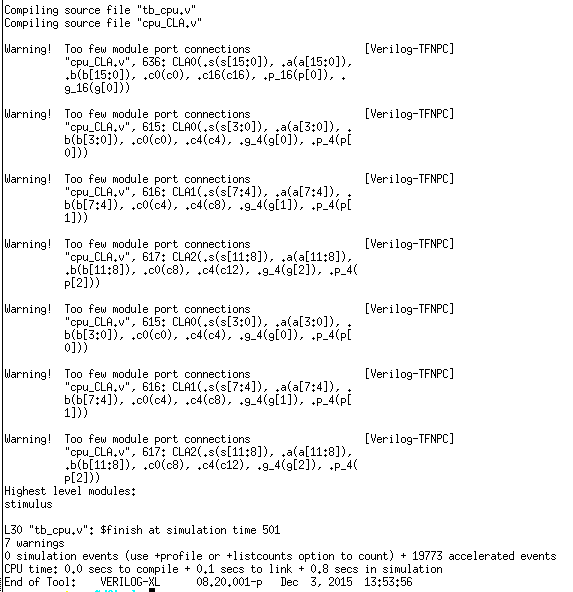
\includegraphics[width=0.7\linewidth]{../CLA/CLA-text}
\caption{Display}
\label{fig:CLA-text}
\end{figure}

\begin{figure}[H]
\centering
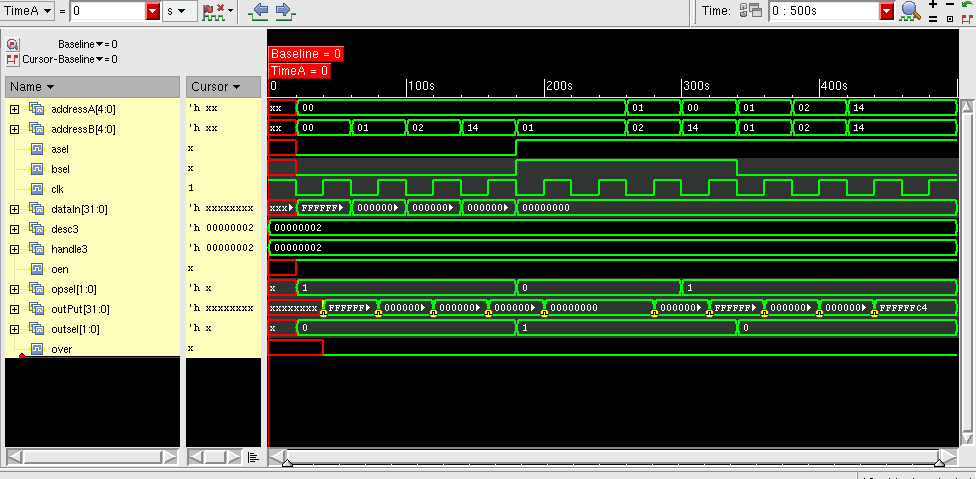
\includegraphics[width=\linewidth]{../CLA/CLA-test}
\caption{Simvision}
\label{fig:CLA-test}
\end{figure}

\subsubsection{Logic Synthesis and Post-Synthesis Simulation}
Figures \ref{fig:synth-text-CRA} and \ref{fig:synth-test-CRA} show the display and simvision results of the simulation. The results are included under the CLA directory under the files \texttt{timing.rep} and \texttt{cell.rep}. They show that this design uses 48610.093084nm of area and has a slack time of 26.14 meaning that the clock rate can be increased.
\begin{figure}[H]
\centering
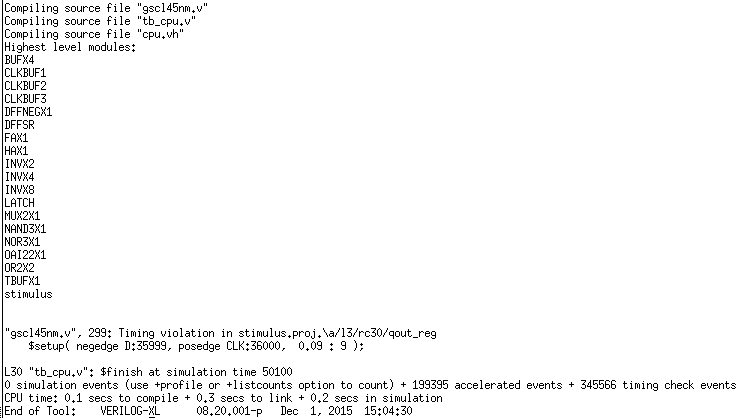
\includegraphics[width=.7\linewidth]{../CLA/synth-text}
\caption{Display}
\label{fig:synth-text-CLA}
\end{figure}

\begin{figure}[H]
\centering
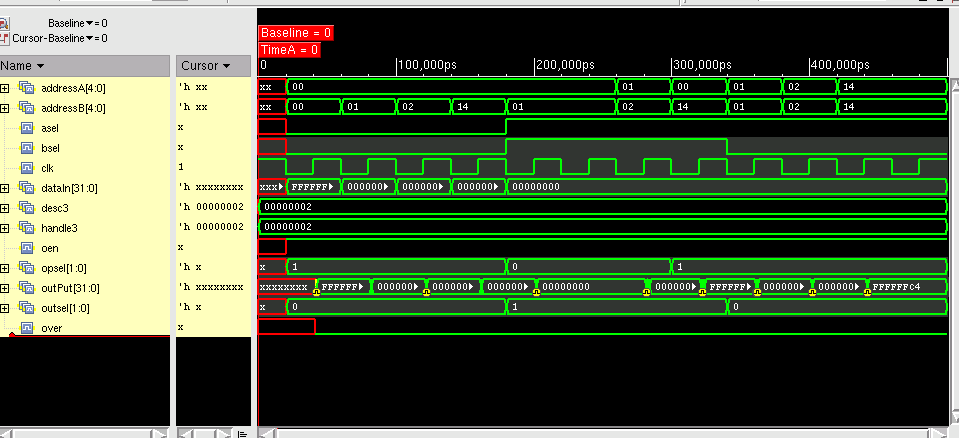
\includegraphics[width=\linewidth]{../CLA/synth-test}
\caption{Simvision}
\label{fig:synth-test-CLA}
\end{figure}


\subsubsection{Place \& Route and Post-P\&R Simulation}
Figures \ref{fig:encounter-text-CLA} and \ref{fig:encounter-test-CLA} show the display and simvision results. The file \texttt{timing.rep.5.final} is located under the CLA directory included with this report. It shows that the slack time is about 17.921 which is an improvement from the post-synthesis design, but the clock can still be increased. The max clock rate was found to be $\approx$ 66 MHz.
\begin{figure}[H]
\centering
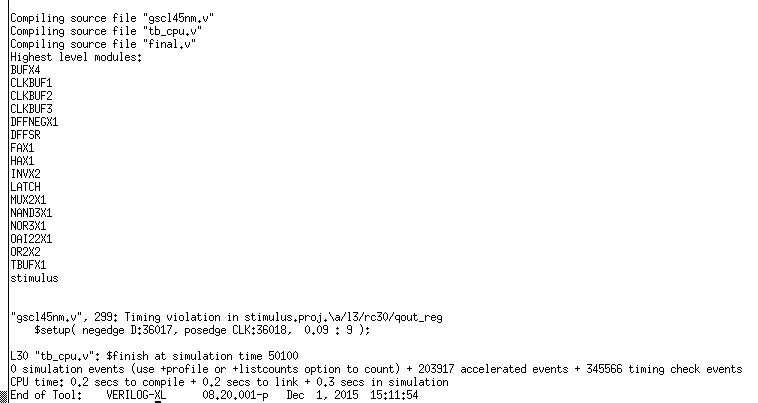
\includegraphics[width=.7\linewidth]{../CLA/encounter-text}
\caption{Display}
\label{fig:encounter-text-CLA}
\end{figure}

\begin{figure}[H]
\centering
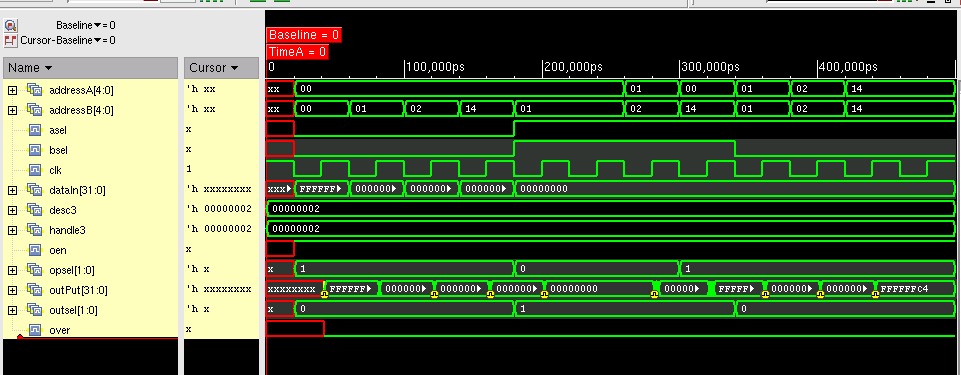
\includegraphics[width=\linewidth]{../CLA/encounter-test}
\caption{Simvision}
\label{fig:encounter-test-CLA}
\end{figure}

\subsubsection{Test Bench}
Figures \ref{fig:test-text-CLA} and \ref{fig:test-test-CLA} show the display and simvision results. For a detailed analysis of the output please refer to the file \texttt{stim\_proj\_CLA.out} located under the CRA directory included with this report. Figures  \ref{fig:alu1-CLA} and \ref{fig:alu2-CLA} show a detailed view of the ALU results.
\begin{figure}[H]
\centering
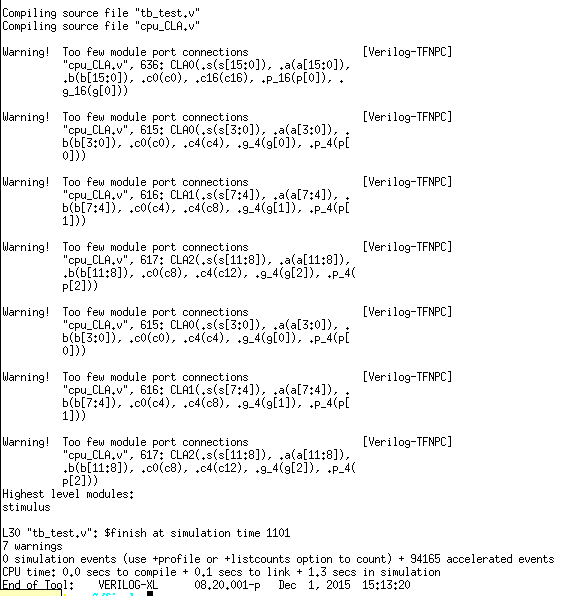
\includegraphics[width=.7\linewidth]{../CLA/test-text}
\caption{RTL Display}
\label{fig:test-text-CLA}
\end{figure}


\begin{figure}[H]
\centering
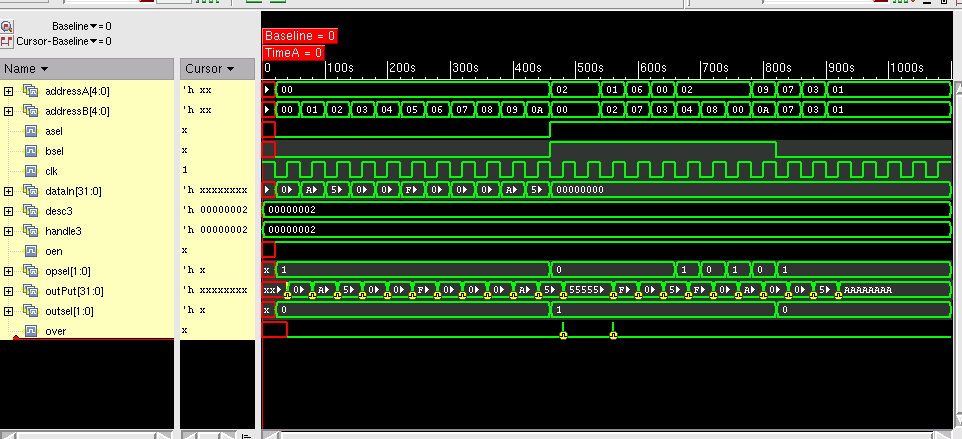
\includegraphics[width=\linewidth]{../CLA/test-test}
\caption{RTL Simvision}
\label{fig:test-test-CLA}
\end{figure}

\begin{figure}[H]
\centering
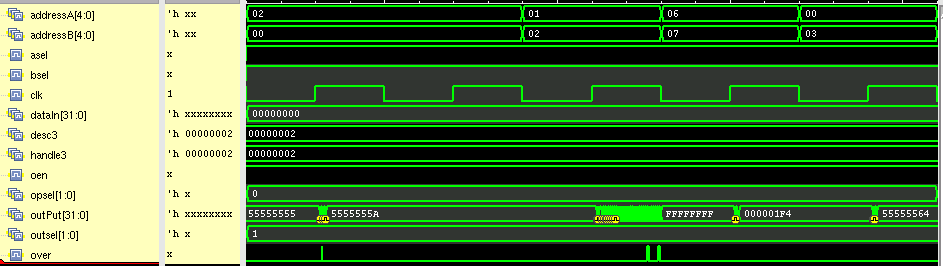
\includegraphics[width=\linewidth]{../CLA/alu1}
\caption{ALU 1}
\label{fig:alu1-CLA}
\end{figure}

\begin{figure}[H]
\centering
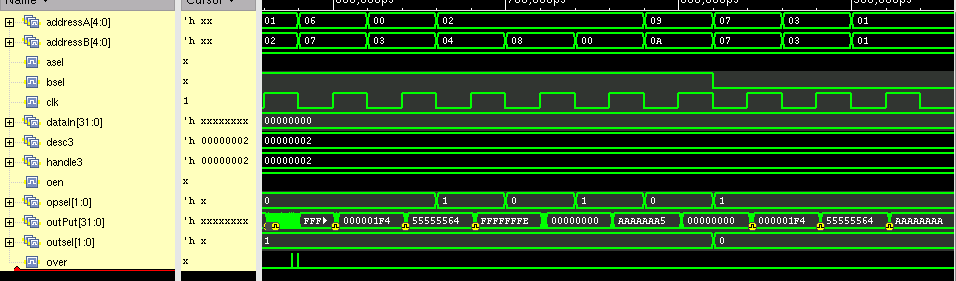
\includegraphics[width=\linewidth]{../CLA/alu2}
\caption{ALU 2}
\label{fig:alu2-CLA}
\end{figure}



\subsection{Carry Skip Adder}
In the Carry Skip Adder, the operands are divided into blocked of r bits blocks. In each block, a ripple carry adder can be utilized to produce the sum bits and a carryout bit for the block. This is shown in Figure \ref{fig:carry-skip}.

\begin{figure}[H]
\centering
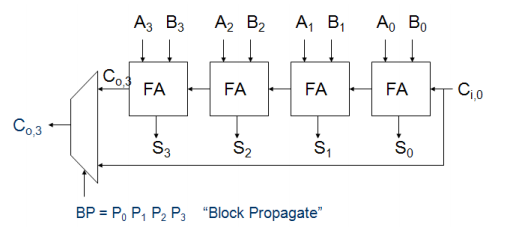
\includegraphics[width=0.7\linewidth]{carry-skip}
\caption{Carry Skip Adder}
\label{fig:carry-skip}
\end{figure}

\subsubsection{RTL Simulation}
Figures \ref{fig:RTL-text-CSA} and \ref{fig:CSA-test} show the display and simvision results of the RTL simulation. The detailed results are included with this report under the CSA directory in the file \texttt{stim\_proj.out}.
\begin{figure}[H]
	\centering
	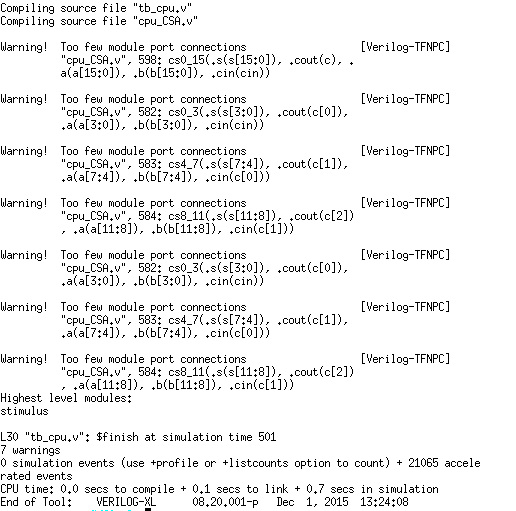
\includegraphics[width=.7\linewidth]{../CSA/RTL-text}
	\caption{Display}
	\label{fig:RTL-text-CSA}
\end{figure}


\begin{figure}[H]
	\centering
	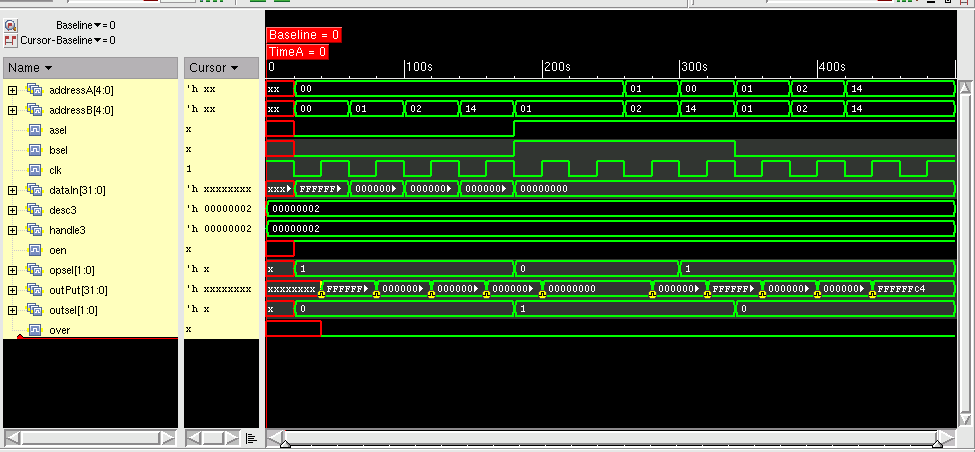
\includegraphics[width=\linewidth]{../CSA/CSA-test}
	\caption{Simvision}
	\label{fig:CSA-test}
\end{figure}
\subsubsection{Logic Synthesis and Post-Synthesis Simulation}
Figures \ref{fig:synth-text-CSA} and \ref{fig:synth-test-CSA} show the display and simvision results of the simulation. The results are included under the CSA directory under the files \texttt{timing.rep} and \texttt{cell.rep}. They show that this design uses 48878.063377nm of area and has a slack time of 26.14 meaning that the clock rate can be increased.

\begin{figure}[H]
\centering
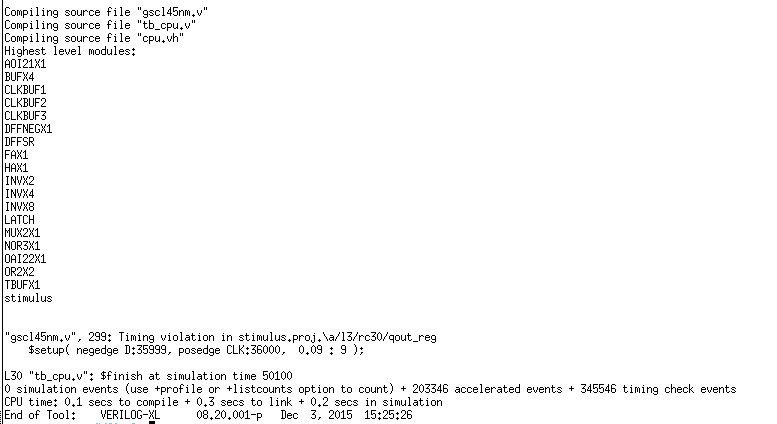
\includegraphics[width=\linewidth]{../CSA/synth-text-CSA}
\caption{Display}
\label{fig:synth-text-CSA}
\end{figure}


\begin{figure}[H]
\centering
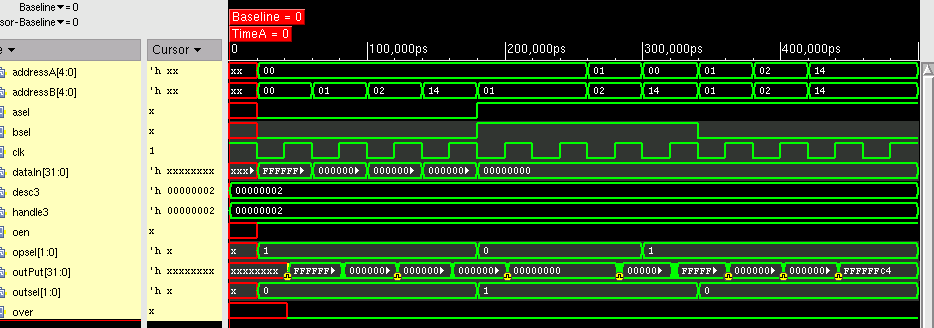
\includegraphics[width=\linewidth]{../CSA/synth-test-CSA}
\caption{Simvision}
\label{fig:synth-test-CSA}
\end{figure}

\subsubsection{Place \& Route and Post-P\&R Simulation}
Figures \ref{fig:EC-text-CSA} and \ref{fig:EC-test-CSA} show the display and simvision results. The file \texttt{timing.rep.5.final} is located under the CSA directory included with this report. It shows that the slack time is about 18.318 which is an improvement from the post-synthesis design, but the clock can still be increased. The max clock rate was found to be $\approx$ 66 MHz.
\begin{figure}[H]
\centering
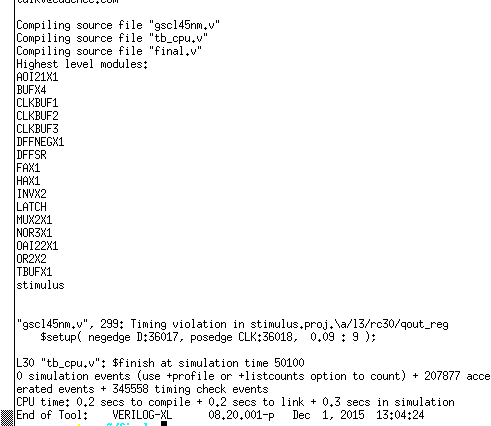
\includegraphics[width=.7\linewidth]{../CSA/EC-text}
\caption{Display}
\label{fig:EC-text-CSA}
\end{figure}
\begin{figure}[H]
\centering
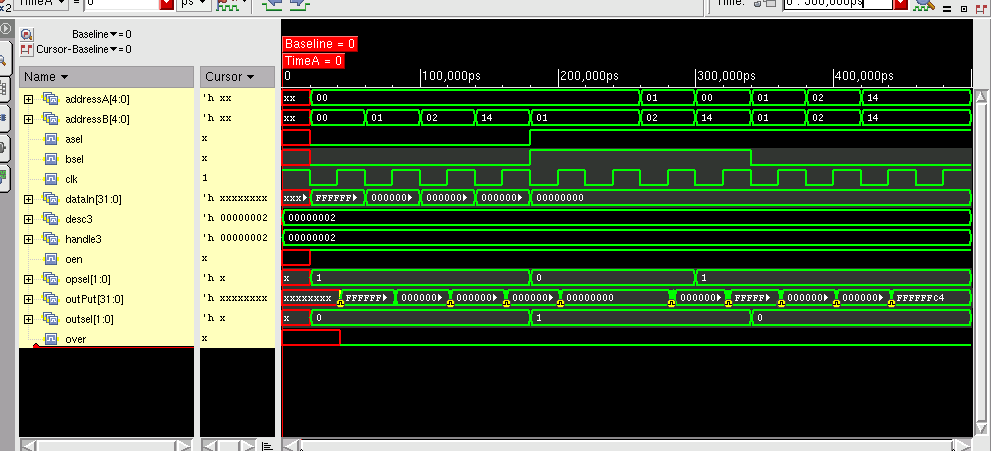
\includegraphics[width=.7\linewidth]{../CSA/EC}
\caption{Simvision}
\label{fig:EC-test-CSA}
\end{figure}

\subsubsection{Test Bench}
Figures \ref{fig:test-text-CSA} - \ref{fig:test2-test-CSA} show the display and simvision results. For a detailed analysis of the output please refer to the file \texttt{stim\_proj\_CSA.out} located under the CSA directory included with this report.
\begin{figure}[H]
\centering
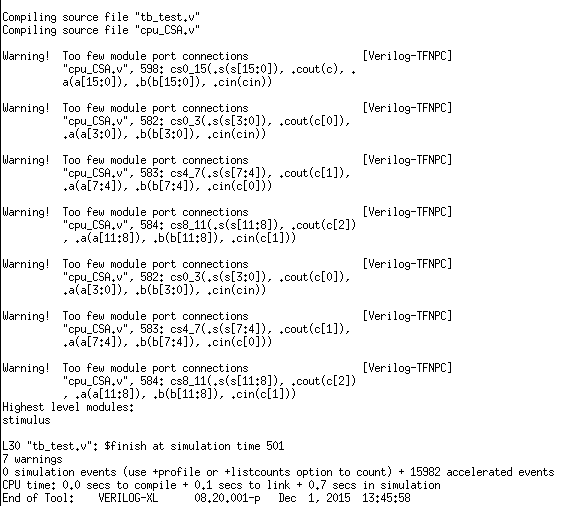
\includegraphics[width=.7\linewidth]{../CSA/tbtest-text}
\caption{Display}
\label{fig:test-text-CSA}
\end{figure}
\begin{figure}[H]
\centering
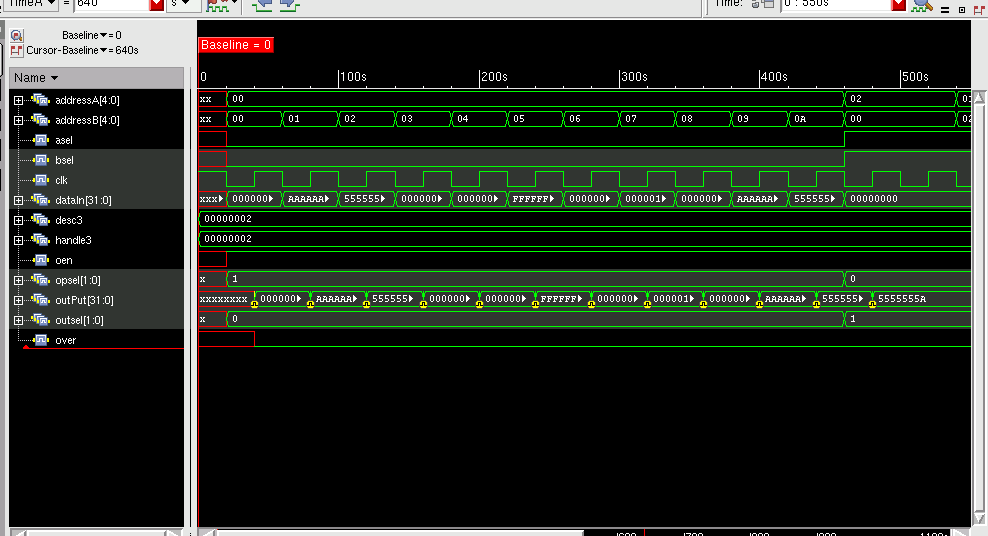
\includegraphics[width=\linewidth]{../CSA/test1}
\caption{Simvision 1}
\label{fig:test1-test-CS}
\end{figure}
\begin{figure}[H]
\centering
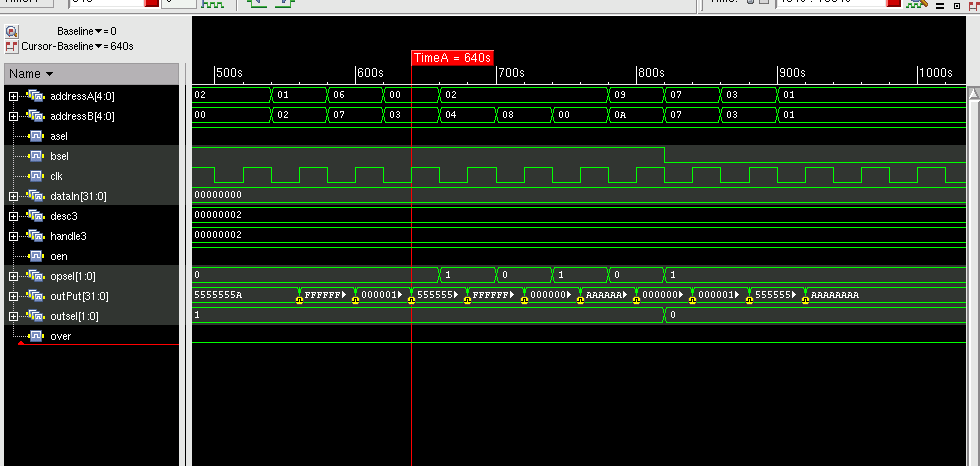
\includegraphics[width=\linewidth]{../CSA/test2}
\caption{Simvision 2}
\label{fig:test2-test-CSA}
\end{figure}

\subsection{Carry Select Adder}
The Carry Select Adder divides the operands to be added into r bit blocks similar to the Carry Skip Adder. For each block, two r-bit Ripple Carry Adders operate in parallel to form two sets of sum bits and carry out signals. Each Ripple Carry Adder has two sets of hard-coded carry-in signals. One Ripple Carry Adder has a carry-in of 0, while the other has a carry-in of 1. This is shown in Figure \ref{fig:carry-select}.

\begin{figure}[H]
\centering
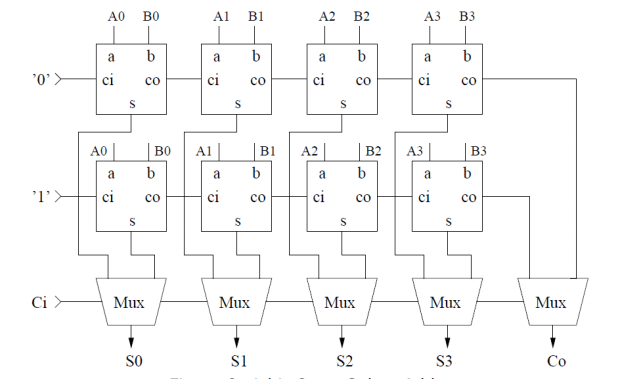
\includegraphics[width=0.7\linewidth]{carry-select}
\caption{Carry Select Adder}
\label{fig:carry-select}
\end{figure}

\subsubsection{RTL Simulation}
Figures \ref{fig:CSeA-text} and \ref{fig:CSeA-test} show the display and simvision results of the RTL simulation. The detailed results are included with this report under the CSeA directory in the file \texttt{stim\_proj.out}.
\begin{figure}[H]
\centering
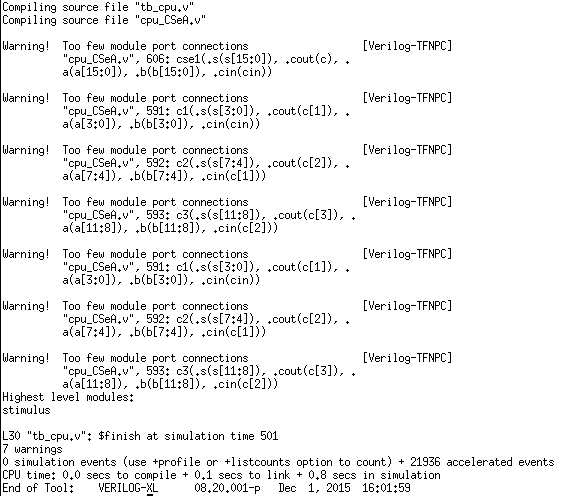
\includegraphics[width=.7\linewidth]{../CSeA/CSeA-text}
\caption{Display}
\label{fig:CSeA-text}
\end{figure}

\begin{figure}[H]
\centering
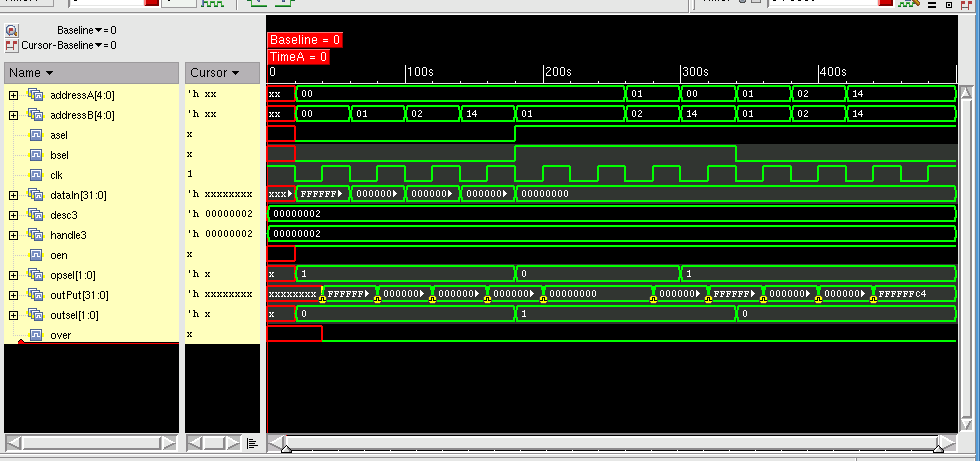
\includegraphics[width=\linewidth]{../CSeA/CSeA-test}
\caption{Simvision}
\label{fig:CSeA-test}
\end{figure}

\subsubsection{Logic Synthesis and Post-Synthesis Simulation}
Figures \ref{fig:synth-text-CSeA} and \ref{fig:synth-test-CSeA} show the display and simvision results of the simulation. The results are included under the CSA directory under the files \texttt{timing.rep} and \texttt{cell.rep}. They show that this design uses 49150.726672nm of area and has a slack time of 26.14 meaning that the clock rate can be increased.
\begin{figure}[H]
\centering
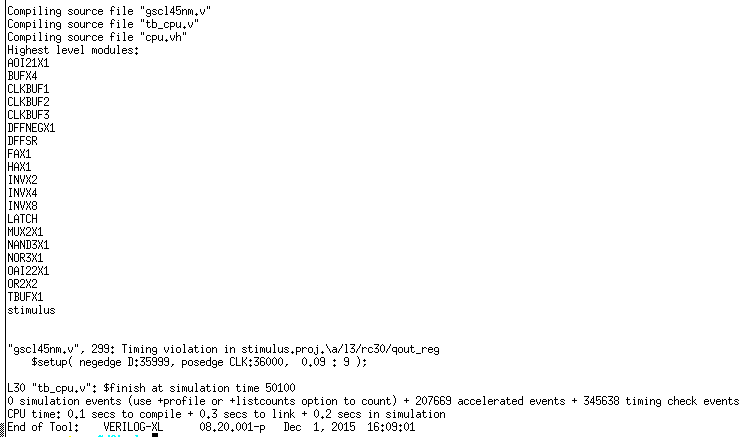
\includegraphics[width=.7\linewidth]{../CSeA/synth-text}
\caption{Display}
\label{fig:synth-text-CSeA}
\end{figure}
\begin{figure}[H]
\centering
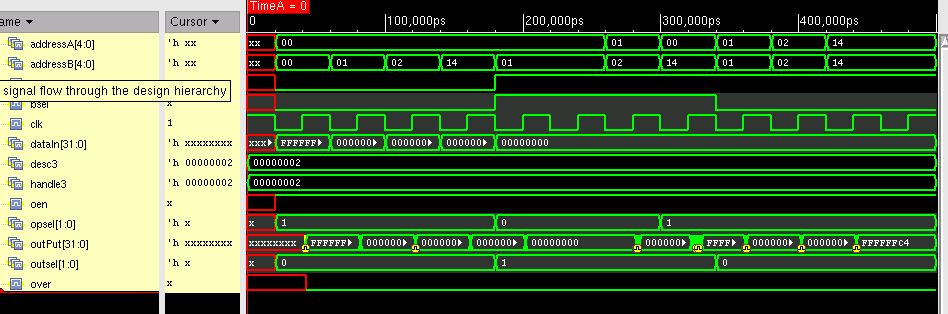
\includegraphics[width=\linewidth]{../CSeA/synth-test}
\caption{Simvision}
\label{fig:synth-test-CSeA}
\end{figure}

\subsubsection{Place \& Route and Post-P\&R Simulation}
Figures \ref{fig:EC-text-CSeA} and \ref{fig:EC-test-CSeA} show the display and simvision results. The file \texttt{timing.rep.5.final} is located under the CSeA directory included with this report. It shows that the slack time is about 18.144 which is an improvement from the post-synthesis design, but the clock can still be increased. The max clock rate was found to be $\approx$ 66 MHz.
\begin{figure}[H]
\centering
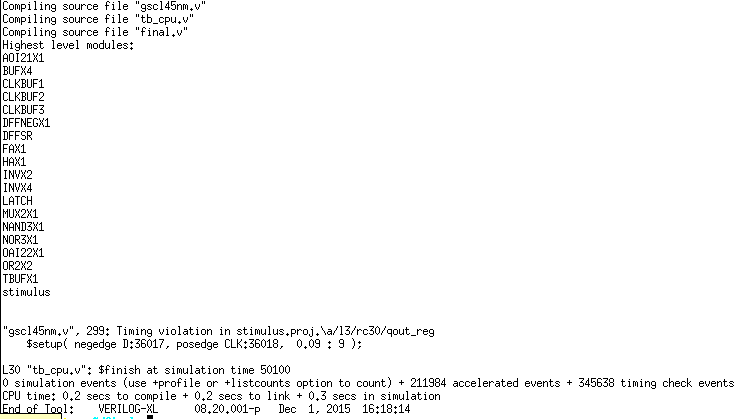
\includegraphics[width=.7\linewidth]{../CSeA/encounter-text}
\caption{Display}
\label{fig:EC-text-CSeA}
\end{figure}
\begin{figure}[H]
\centering
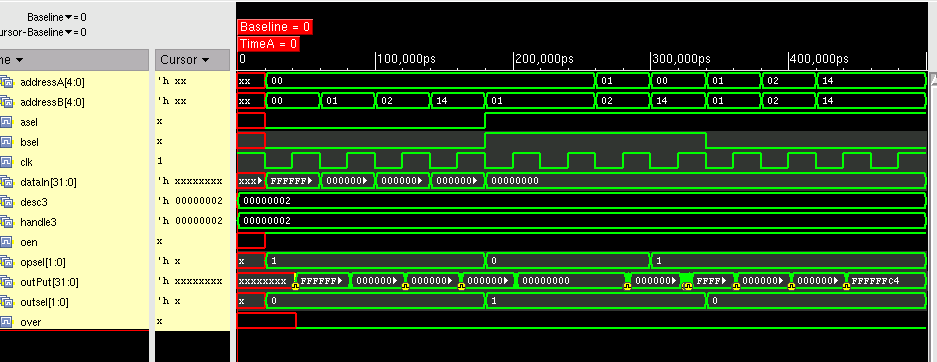
\includegraphics[width=\linewidth]{../CSeA/encounter-test}
\caption{Simvision}
\label{fig:EC-test-CSeA}
\end{figure}

\subsubsection{Test Bench}
Figures \ref{fig:test-text-CSeA} and \ref{fig:test-test-CSeA} show the display and simvision results. For a detailed analysis of the output please refer to the file \texttt{stim\_proj\_CSeA.out} located under the CSeA directory included with this report. Figures  \ref{fig:alu1-CSeA} and \ref{fig:alu2-CSeA} show a detailed view of the ALU results.
\begin{figure}[H]
\centering
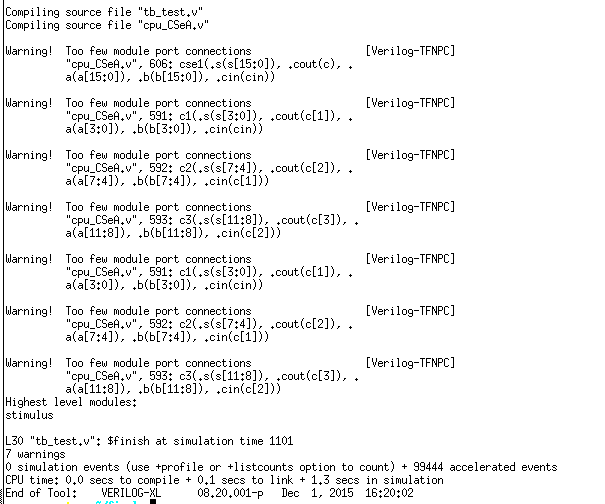
\includegraphics[width=.7\linewidth]{../CSeA/test-text}
\caption{Display}
\label{fig:test-text-CSeA}
\end{figure}
\begin{figure}[H]
\centering
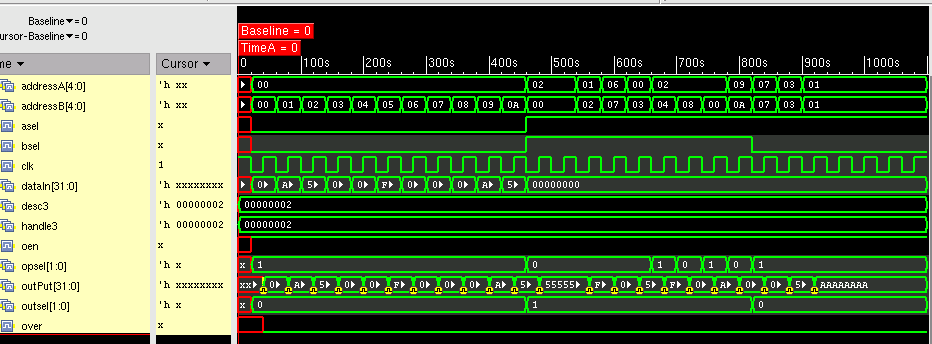
\includegraphics[width=\linewidth]{../CSeA/test-test}
\caption{Simvision}
\label{fig:test-test-CSeA}
\end{figure}


\begin{figure}[H]
\centering
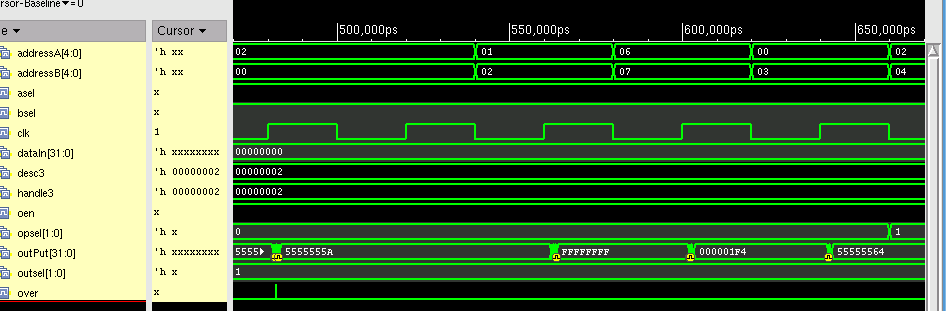
\includegraphics[width=\linewidth]{../CSeA/alu1}
\caption{ALU Operations 1}
\label{fig:alu1-CSeA}
\end{figure}
\begin{figure}[H]
\centering
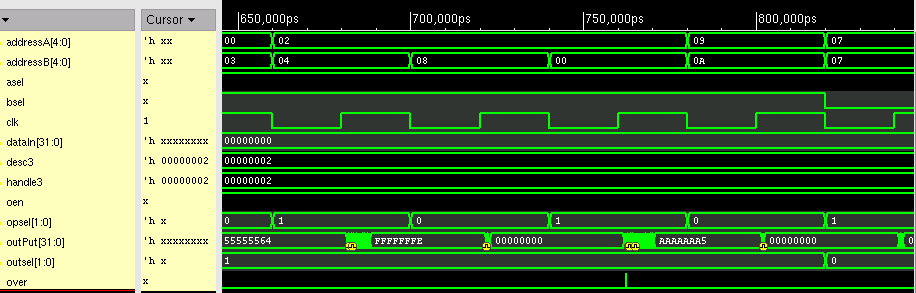
\includegraphics[width=\linewidth]{../CSeA/alu2}
\caption{ALU Operations 2}
\label{fig:alu2-CSeA}
\end{figure}

\subsection{Delay Comparison}

\begin{table}[H]
	\begin{center}
		\begin{tabular}{ |c|c|c|c|c| }
			\hline
			Operation & CRA & CLA & CSA & CSeA \\

			\hline
			5555\_5555 + 0000\_0005 & 23.1ns & 23.2ns & 23.6ns & 23.6ns \\
			\hline
			AAAA\_AAAA + 5555\_5555 & 25.2ns & 40.2ns& 28.1ns& 23.9ns \\
			\hline
			0000\_00C8 + 0000\_012C & 22.9ns & 22.5ns &  23.4ns& 23.4ns \\
			\hline
			5555\_555A + 0000\_000A & 23.1ns & 22.8ns & 22.9ns & 23.7ns \\
			\hline
			FFFF\_FFFF - 0000\_0001 & 22.9ns & 22.8ns & 23.3ns & 28.5ns \\
			\hline
			FFFF\_FFFF + 0000\_0001 & 40.8ns & 22.9ns & 30.4ns & 23.1ns \\
			\hline
			FFFF\_FFFF - 5555\_555A & 24.1ns & 22.2ns & 24.6ns & 30.1ns \\
			\hline
			AAAA\_AAAB + 5555\_5555 & 22.1ns & 22.1ns & 25.2ns & 23.2ns \\
			\hline
		\end{tabular}
	\end{center}
	\caption{Width of 180nm}
	\label{tab:2nd}
\end{table}

Overall each adder performed reasonably well. It should be noted that some adders had longer delays on some operations than others. This has to due with how they each algorithmically perform operations. It should be noted that the Carry Select Adder performed the best on average.
\subsection{New Test Bench Code}
This code for \texttt{tb\_test.v} is displayed below and is also included under the directory code included with this report.
\lstinputlisting{tb_test.v}

\section{32-Bit CPU Design with New ALU Architecture}
\subsection{Code}
Below is the code developed to include the 32-bit comparator in the CPU.
\lstinputlisting[firstnumber=1935,firstline=1935, lastline=2076]{cpu_comp.v}


The file \texttt{tb\_test\_comp.v} is not included in this report due to the length. It is included separately with the report under the directory code.
\subsection{RTL Test Bench}
Figures \ref{fig:rtl-results1} - \ref{fig:rtl-results4} show the RTL simulation simvision results of \texttt{tb\_test\_comp.v}, which is included in under the code directory included with this report. The results are also included in the file \texttt{stim\_proj.out} under the directory case2.
\begin{figure}[H]
\centering
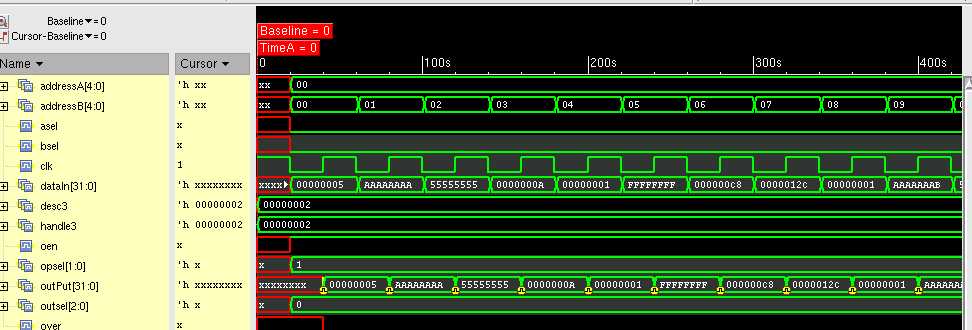
\includegraphics[width=\linewidth]{../case2/rtl-results1}
\caption{Test Bench 1}
\label{fig:rtl-results1}
\end{figure}
\begin{figure}[H]
\centering
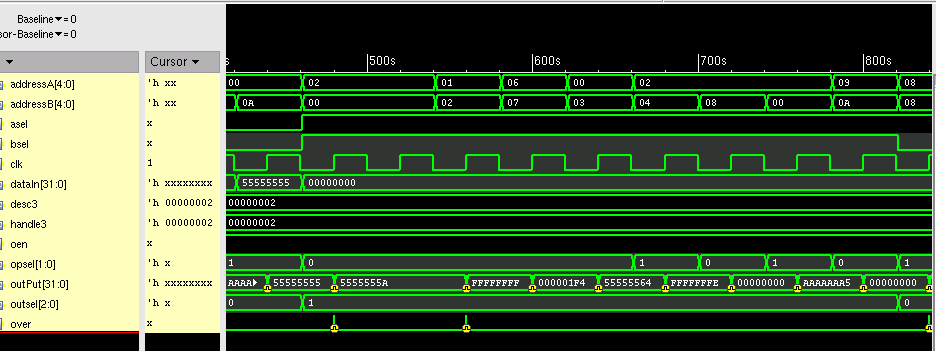
\includegraphics[width=\linewidth]{../case2/rtl-results2}
\caption{Test Bench 2}
\label{fig:rtl-results2}
\end{figure}
\begin{figure}[H]
\centering
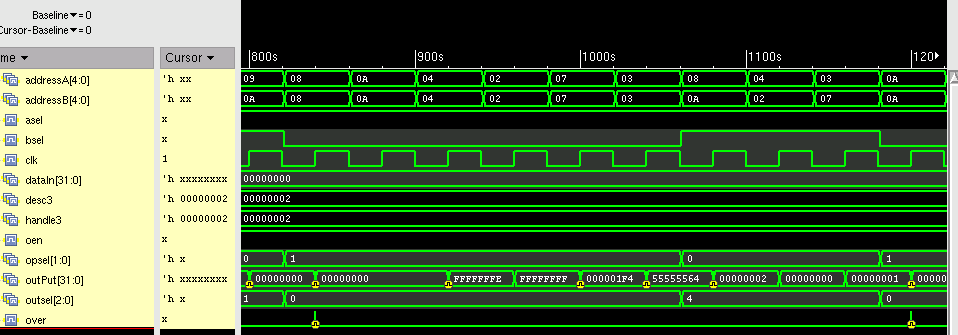
\includegraphics[width=\linewidth]{../case2/rtl-results3}
\caption{Test Bench 3}
\label{fig:rtl-results3}
\end{figure}
\begin{figure}[H]
\centering
\includegraphics[width=\linewidth]{../case2/rtl-results4}
\caption{Test Bench 4}
\label{fig:rtl-results4}
\end{figure}


\subsubsection{Logic Synthesis and Post-Synthesis Simulation}
The results of the post synthesis simulation simvision results are shown in Figures \ref{fig:synth1} - \ref{fig:synth4}. The area of this design is 49305.595675nm and the slack is 26.48. The results of \texttt{timing.rep} and \texttt{timing.cell} are included with this report under the directory case2.
\begin{figure}[H]
\centering
\includegraphics[width=\linewidth]{../case2/synth1}
\caption{Synthesis Simulation 1}
\label{fig:synth1}
\end{figure}
\begin{figure}[H]
\centering
\includegraphics[width=\linewidth]{../case2/synth2}
\caption{Synthesis Simulation 2}
\label{fig:synth2}
\end{figure}
\begin{figure}[H]
\centering
\includegraphics[width=\linewidth]{../case2/synth3}
\caption{Synthesis Simulation 3}
\label{fig:synth3}
\end{figure}
\begin{figure}[H]
\centering
\includegraphics[width=\linewidth]{../case2/synth4}
\caption{Synthesis Simulation 4}
\label{fig:synth4}
\end{figure}


\subsubsection{Place \& Route and Post-P\&R Simulation}
The results of the post-P\&R simulation simvision results are shown in Figures \ref{fig:power} - \ref{fig:enc4}. The results of \texttt{timing.rep.5.final} show a slack of 19.848. This file is included under the directory case2. The maximum clock frequency was found to be $\approx$ 71 MHz.
\begin{figure}[H]
\centering
\includegraphics[width=.7\linewidth]{../case2/power}
\caption{Power Consumption}
\label{fig:power}
\end{figure}

\begin{figure}[H]
\centering
\includegraphics[width=\linewidth]{../case2/enc1}
\caption{Layout Simulation 1}
\label{fig:enc1}
\end{figure}
\begin{figure}[H]
\centering
\includegraphics[width=\linewidth]{../case2/enc2}
\caption{Layout Simulation 2}
\label{fig:enc2}
\end{figure}
\begin{figure}[H]
\centering
\includegraphics[width=\linewidth]{../case2/enc3}
\caption{Layout Simulation 3}
\label{fig:enc3}
\end{figure}
\begin{figure}[H]
\centering
\includegraphics[width=\linewidth]{../case2/enc4}
\caption{Layout Simulation 4}
\label{fig:enc4}
\end{figure}


\section{Conclusions}
Overall a 32-bit pipelined CPU was successfully studied. Through the simulation and analysis of the code, it is clear how a CPU is both physically and logically constructed. Different adder types were adequately analyzed and it is apparent that each configuration affects the power and delay of the CPU as a whole. Furthermore, a comparator was successfully added to the ALU of the CPU. The goals of this project were all achieved successfully.



\end{document}
